\chapter{Przekształcenia geometryczne w przestrzeni}

\textit{Przekształceniem geometrycznym} lub \textit{odwzorowaniem geometrycznym} nazywamy funkcję, której dziedziną i przeciwdziedziną jest zbiór wszystkich punktów przestrzeni $\mathbb{R}^{n}$. W węższym znaczeniu jest to funkcja wzajemnie jednoznaczna przekształcająca jeden zbiór punktów, zwany \textit{figurą geometryczną} lub \textit{wektorem} w inny obiekt tego samego typu.\footnote{Źródło: https://www.math.edu.pl/przeksztalcenia-w-przestrzeni [Dostęp: 26.01.22]} 

\section{Definicja macierzy}
Układ $m \cdot n$ elementów $a_{ij} \in \mathbb{R}$ $(i = 1,\cdots,m, j = 1,\cdots,n)$ zapisany w następującej postaci:
\begin{equation*}
    \begin{bmatrix}
    a_{11} & \cdots & a_{1n} \\
    \cdots & \cdots & \cdots \\
    a_{m1} & \cdots & a_{mn}
    \end{bmatrix}
\end{equation*}
nazywamy macierzą o $m$ wierszach i $n$ kolumnach zdefiniowaną nad ciałem $\mathbb{R}$ (lub macierzą wymiaru $m \times n$). \citep[s. 85]{Repetytorium1977}.
Macierz można też zapisywać krócej:
\begin{equation*}
\mathbb{A} = [a_{i,j}]_{m\times n}    
\end{equation*}

Liczby zawarte w macierzy nazywamy jej \textit{elementami} (zob. rys. 23) \citep[s. 18]{Rutkowski_2008}.

\begin{figure}[H]
\begin{equation*}
\mathbb{A} =
    \begin{bmatrix}
    1 & 2 \\
    3 & 4 \\
    1 & 0
    \end{bmatrix}
\end{equation*}
\centering
\caption{Macierz prostokątna $\mathbb{A }$ wymiaru $3 \times 2$.}
\end{figure}

Macierz o wymiarach $n \times n$ nazywamy \textit{macierzą kwadratową stopnia n} (zob. rys. 24).

\begin{figure}[H]
\begin{equation*}
\mathbb{B} =
    \begin{bmatrix}
    1 & 2 & 3 & 4 \\
    5 & 6 & 7 & 8 \\
    9 & 10 & 11 & 12 \\
    13 & 14 & 15 & 16
    \end{bmatrix}
\end{equation*}
\centering
\caption{Macierz kwadratowa $\mathbb{B}$ wymiaru $4 \times 4$. Macierz kwadratowa ma taką samą liczbę wierszy i kolumn.}
\end{figure}

Odwołanie się do elementu macierzy następuje poprzez nazwę macierzy wraz z towarzyszącym jej dolnym indeksem wierszowym i kolumnowym. Dla przykładowej macierzy $\mathbb{A}_{3\times3}$ indeksy elementów wyglądają następująco:

\begin{equation*}
\mathbb{A}_{3\times3} =
    \begin{bmatrix}
    \mathbf{a_{11}} & a_{12} & a_{13} \\
    a_{21} & \mathbf{a_{22}} & a_{23} \\
    a_{31} & a_{32} & \mathbf{a_{33}}
    \end{bmatrix}
\end{equation*}
Pogrubieniem oznaczono tak zwaną \textit{przekątną główną macierzy}, którą tworzą elementy o równych wartościach indeksów wierszowych i kolumnowych.

\textit{Wektorem wierszowym} nazywamy macierz złożoną tylko z jednego wiersza. Na przykład:

\begin{equation*}
    \mathbb{A}_{1\times3} =
    \begin{bmatrix}
   1 & 2 & 3
    \end{bmatrix}
\end{equation*}

Analogicznie, \textit{wektorem kolumnowym} nazywamy macierz złożoną tylko  z pojedynczej kolumny:
\begin{equation*}
    \mathbb{A}_{3\times1} =
    \begin{bmatrix}
    1 \\ 2 \\ 3
    \end{bmatrix}
\end{equation*}

\section{Iloczyn macierzy}
\begin{definicja}
Iloczynem macierzy\footnote{Opracowano na podstawie \citep[s. 88]{Repetytorium1977}}
\begin{equation*}
\begin{bmatrix}
a_{11} & \cdots & a_{1n} \\
\vdots \\
a_{m1} & \cdots & a_{mn}
\end{bmatrix}
\in \mathbb{M}_{m \times n} \quad ,
\begin{bmatrix}
b_{11} & \cdots & b_{1p} \\
\vdots \\
b_{n1} & \cdots & b_{np}
\end{bmatrix}
\in \mathbb{M}_{n \times p} 
\end{equation*}
nazywamy macierz
\begin{equation*}
\begin{bmatrix}
c_{11} & \cdots & c_{1p} \\
\vdots \\
c_{m1} & \cdots & c_{mp}
\end{bmatrix}
\in \mathbb{M}_{m \times p} \, ,
\end{equation*}
gdzie 
\begin{equation*}
    c_{ij} = \sum^{n}_{k=1} a_{ik} b_{kj}
\end{equation*}
i piszemy
\begin{equation*}
    [c_{ij}] = [a_{ij}] \cdot [b_{ij}] \ \text{lub} \ [a_{ij}][b_{ij}].
\end{equation*}
\end{definicja}
\begin{przyklad}

Załóżmy, że mamy dwie macierze, macierz $\mathbb{A}_{2 \times 3}$ i macierz $\mathbb{B}_{3\times 2}$. Po ich pomnożeniu otrzymamy nową macierz $\mathbb{C}$, która posiada tyle wierszy ile miała macierz $\mathbb{A}$ i tyle kolumn ile miała macierz $\mathbb{B}$. Zatem w tym wypadku macierz $\mathbb{C}$ ma 2 wiersze i 2 kolumny. 
Zatem mnożenie:
\begin{equation*}
    \mathbb{A}_{2 \times 3} =
    \begin{bmatrix}
    1 & 2 & 3 \\
    4 & 5 & 6
    \end{bmatrix}
    ,\quad  
    \mathbb{B}_{3 \times 2} =
    \begin{bmatrix}
    1 & 3 \\
    2 & 4 \\
    1 & 2
    \end{bmatrix}
\end{equation*}
daje nam:
\begin{equation*}
    \mathbb{C}_{2\times 2} =
    \begin{bmatrix}
    1 \cdot 1 + 2 \cdot 2 + 3 \cdot 1 & 1 \cdot 3 + 2 \cdot 4 + 3 \cdot 2 \\
    4 \cdot 1 + 5 \cdot 2 + 6 \cdot 1 & 4 \cdot 3 + 5 \cdot 4 + 6 \cdot 2
    \end{bmatrix}
    =
    \begin{bmatrix}
    8 & 17 \\
    20 & 44
    \end{bmatrix}
\end{equation*}.
\end{przyklad}

Jak można zauważyć macierz $\mathbb{C}$ jest sumą iloczynów kolejnych elementów z każdego wiersza macierzy $\mathbb{A}$ przez każdy kolejny element z każdej kolumny macierzy $\mathbb{B}$.
Operacja mnożenia macierzy jest przydatna do wyznaczenia tzw. \textit{Macierzy obrotu}.




\subsection{Macierz obrotu}
Macierz obrotu to szczególny rodzaj macierzy, umożliwiający poprzez mnożenie z  danym wektorem $v$ wymiaru $n$ uzyskanie nowego wektora $v'$ obróconego o zadany kąt $\phi$ względem początku układu współrzędnych umieszczonego nad ciałem $\mathbb{R}^{n}$.\footnote{Źródło: \url{https://www.obliczeniowo.com.pl/258}}

\section{Obroty w \texorpdfstring{$\mathbb{R}^{2}$}{Obroty w R2}}

\begin{figure}[H]
    \centering
    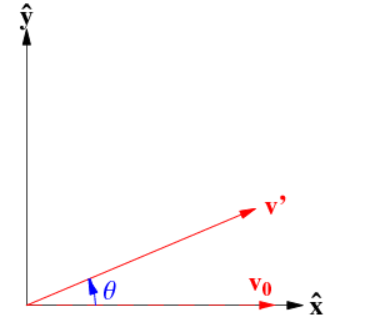
\includegraphics[scale=0.8]{RotationMatrix.png}
    \caption{ Obrót wektora $v_{0}$ o kąt $\phi$ względem osi $x$. Za: \citep{Weisstein2000}.}
\end{figure}

Macierz obrotu w $\mathbb{R}^{2}$ oznaczamy zwykle symbolem $R(\phi)$\footnote{Za: \citep{Weisstein2000}.}:

\begin{equation*}
R(\phi) =
    \begin{bmatrix}
    \cos\phi & -\sin\phi \\
    \sin\phi & \cos\phi
    \end{bmatrix}
\end{equation*}
Zatem:
\begin{equation*}
    v' = R_{\phi} \cdot v_{0}.
\end{equation*}
Obrót wektora w $\mathbb{R}^{2}$ można wtedy wykonać poprzez zwykłe mnożenie macierzowe w następujący sposób:

\begin{equation*}
    v = R(\phi) \cdot v =
    \begin{bmatrix}
    \cos\phi & -\sin\phi \\
    \sin\phi & \cos\phi 
    \end{bmatrix}
    \cdot
    \begin{bmatrix}
    x \\
    y
    \end{bmatrix}
    =
    \begin{bmatrix}
    x \cdot \cos\phi & - & y \cdot \sin\phi \\
    x \cdot \sin\phi & + & y \cdot \cos\phi
    \end{bmatrix}
\end{equation*}
Macierz ta obraca wektory kolumnowe w następujący sposób:

\begin{equation*}
v' =
    \begin{bmatrix}
    x' \\
    y
    \end{bmatrix}
    =
    \begin{bmatrix}
    \cos\phi & -\sin\phi \\
    \sin\phi & \cos\phi
    \end{bmatrix}
    \cdot
    \begin{bmatrix}
    x \\
    y
    \end{bmatrix}
\end{equation*}
Wtedy współrzędne wektora:  
\begin{equation*}
v' =
    \begin{bmatrix}
     x' \\
     y'
    \end{bmatrix}
\end{equation*}
mają wartości:
\begin{equation*}
    x' = x \cos\phi - y \sin\phi
\end{equation*},
\begin{equation*}
    y' = x \sin\phi + y \cos\phi
\end{equation*}.

Obrót jest przeciwny do obrotu zgodnego z ruchem wskazówek zegara jeżeli kąt $\phi$ jest dodatni. Macierz obrotu zgodnego z ruchem wskazówek zegara ma postać:

\begin{equation*}
    R(-\phi) =
    \begin{bmatrix}
    \cos\phi & \sin\phi \\
    -\sin\phi & \cos\phi
    \end{bmatrix}
\end{equation*}

Obroty w $\mathbb{R}^{2}$ spełniają własność przemienności. To znaczy, że nie ma znaczenia kolejność wykonywania obrotów. Niezależnie od kolejności otrzymuje się takie same wartości w wektorze wynikowym.
Załóżmy, że mamy wektor:
\begin{equation*}
v =
    \begin{bmatrix}
    1 \\
    0
    \end{bmatrix}
\end{equation*}
\begin{przyklad}
Obróćmy wektor $v$ o kąt $45^{\circ}$ w kierunku zgodnym i przeciwnym do ruchu wskazówek zegara:
\begin{equation*}
    R(45^{\circ}) =
    \begin{bmatrix}
    1 \\
    0
    \end{bmatrix}
    \cdot
    \begin{bmatrix}
    \cos\phi & -\sin\phi \\
    \sin\phi & \cos\phi
    \end{bmatrix}
\end{equation*}
Z tego wynika, że współrzędne wynoszą:
\begin{equation*}
    x' = 1 \cdot \frac{\sqrt{2}}{2} - 0 \cdot \frac{\sqrt{2}}{2}
    = \frac{1}{\sqrt{2}}
\end{equation*}
oraz
\begin{equation*}
    y' = 1 \cdot \frac{\sqrt{2}}{2} + 0 \cdot \frac{\sqrt{2}}{2} = \frac{1}{\sqrt{2}}
\end{equation*}
Zatem otrzymane współrzędne wektora $v'$ przy obrocie w kierunku przeciwnym do ruchu wskazówek zegara wynoszą:
\begin{equation*}
v' =
    \begin{bmatrix}
    \frac{1}{\sqrt{2}} \\
    \frac{1}{\sqrt{2}}
    \end{bmatrix}
\end{equation*}

\begin{equation*}
    R(-45^{\circ}) =
    \begin{bmatrix}
    1 \\
    0
    \end{bmatrix}
    \cdot
    \begin{bmatrix}
    \cos\phi & \sin\phi \\
    -\sin\phi & \cos\phi
    \end{bmatrix}
\end{equation*}
Zatem współrzędne $x'$ i $y'$ wynoszą:
\begin{equation*}
 x' = 1 \cdot -(\frac{\sqrt{2}}{2}) - 0 \cdot -(\frac{\sqrt{2}}{2})
     = -(\frac{1}{\sqrt{2}})
\end{equation*}
\begin{equation*}
     y' = 1 \cdot -(\frac{\sqrt{2}}{2}) + 0 \cdot -(\frac{\sqrt{2}}{2})
     = -(\frac{1}{\sqrt{2}})
\end{equation*}
Otrzymujemy zatem, że współrzędne wektora $v'$ dla obrotu w kierunku zgodnym z kierunkiem ruchu wskazówek zegara wynoszą: 
\begin{equation*}
v' =
    \begin{bmatrix}
    -\frac{1}{\sqrt{2}} \\
    -\frac{1}{\sqrt{2}}
    \end{bmatrix}
\end{equation*}
\end{przyklad}
\section{Obroty w \texorpdfstring{$\mathbb{R}^{3}$}{Obroty w R3} }
Poniżej definiujemy macierze elementarne, które obracają wektor $v$ względem, kolejno: osi $Ox$, $Oy$ oraz $Oz$. Macierze obrotu mają postać:
\begin{equation*}
R_{x}(\phi) =
    \begin{bmatrix}
    1 & 0 & 0 \\
    0 & \cos\phi & -\sin\phi \\
    0 & \sin\phi & \cos\phi 
    \end{bmatrix}
    \end{equation*}
    \\
    \begin{equation*}
    R_{y}(\phi) =
    \begin{bmatrix}
    \cos\phi & 0 & \sin\phi \\
    0 & 1 & 0  \\
    -\sin\phi & 0 & \cos\phi
    \end{bmatrix}
    \end{equation*}
    \\
    \begin{equation*}
        R_{z}(\phi) =
        \begin{bmatrix}
        \cos\phi & -\sin\phi & 0 \\
        \sin\phi & \cos\phi & 0 \\
        0 & 0 & 1
        \end{bmatrix}
    \end{equation*}

\begin{przyklad}
    
Macierz $R_{z}(\phi)$ dla kąta $\phi = 90^{\circ}$ obraca wektor $v$ względem osi $OZ$. Współrzędne wektora $v'$ można wyliczyć dokonując pomnożenia macierzy $R_{z}$ przez wektor $v$ postaci:
\begin{equation*}
v = 
    \begin{bmatrix}
    1 \\
    0 \\
    0
    \end{bmatrix}
\end{equation*}

\begin{equation*}
 R_{z}(90^{\circ}) = 
\begin{bmatrix}
    1 \\
    0 \\ 
    0
    \end{bmatrix}
    \cdot
    \begin{bmatrix}
\cos90^{\circ} & -\sin 90^{\circ} &  0 \\
\sin 90^{\circ} & \cos 90^{\circ} &  0 \\
0 & 0 & 1
    \end{bmatrix}
    = 
    \begin{bmatrix}
    0 & -1 & 0 \\
    1 & 0 & 0 \\
    0 & 0 & 1
    \end{bmatrix}
    \cdot
    \begin{bmatrix}
    1 \\
    0 \\
    0
    \end{bmatrix}
    =
    \begin{bmatrix}
    0 \\
    1 \\
    0
    \end{bmatrix}
\end{equation*}
Analogiczne obliczenia możemy wykonać także dla pozostałych osi.
Oś $OX$:

\begin{equation*}
 R_{x}(90^{\circ}) = 
\begin{bmatrix}
    1 \\
    0 \\ 
    0
    \end{bmatrix}
    \cdot
    \begin{bmatrix}
     1 & 0 & 0 \\
    0 & \cos 90^{\circ} & -\sin90^{\circ} \\
    0 & \sin90^{\circ} & \cos90^{\circ} 
    \end{bmatrix}
    =
    \begin{bmatrix}
     1 \\
     0 \\
     0
    \end{bmatrix}
    \cdot
    \begin{bmatrix}
     1 & 0 & 0 \\
     0 & 0 & -1 \\
     0 & 1 & 0
    \end{bmatrix}
    =
    \begin{bmatrix}
     1 \\
     0 \\
     0
    \end{bmatrix}
\end{equation*}

Oś $OY$:
\begin{equation*}
    R_{y}(90)^{\circ} =
    \begin{bmatrix}
     1 \\
     0 \\
     0
    \end{bmatrix}
    \cdot
    \begin{bmatrix}
     \cos90^{\circ} & 0 & \sin90^{\circ} \\
    0 & 1 & 0  \\
    -\sin90^{\circ} & 0 & \cos90^{\circ}
    \end{bmatrix}
    =
    \begin{bmatrix}
     1 \\
     0 \\
     0
    \end{bmatrix}
    \cdot
    \begin{bmatrix}
     0 & 0 & 1 \\
     0 & 1 & 0 \\
     -1 & 0 & 0
    \end{bmatrix}
    =
    \begin{bmatrix}
     0 \\
     0 \\
     -1
    \end{bmatrix}
\end{equation*}
\end{przyklad}

\begin{figure}[H]
    \centering
    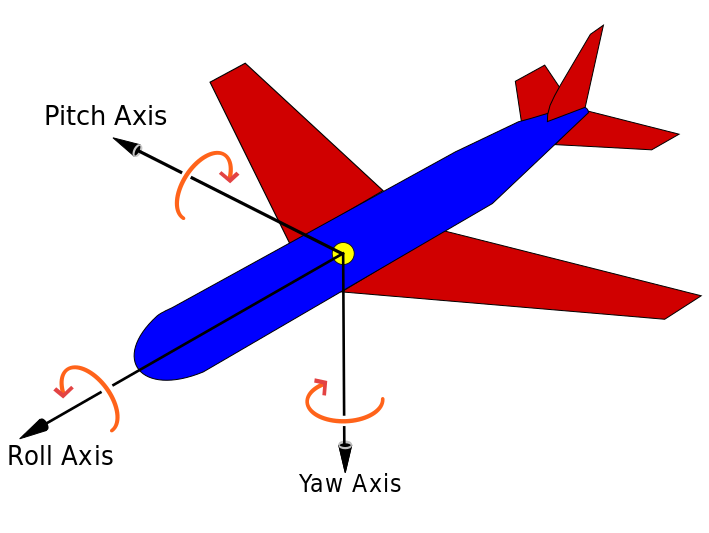
\includegraphics[scale=0.3]{Yaw_Axis_Corrected.png}
    \centering
    \caption{Na rysunku widać położenie trzech osi obrotu: $Ox$, $Oy$ i $Oz$ wraz z towarzyszącymi im kątami. Źródło: \url{https://pl.wikipedia.org/wiki/Macierz_obrotu} [Dostęp: 11.01.22]}
\end{figure}



